% $Id$
% !Mode:: "TeX:DE"    % Setting document mode and submode for WinEdt
% ............................................................................
%             V E R S C H L U E S S E L U N G S V E R F A H R E N
% ~~~~~~~~~~~~~~~~~~~~~~~~~~~~~~~~~~~~~~~~~~~~~~~~~~~~~~~~~~~~~~~~~~~~~~~~~~~~

\begin{refsegment}

% HACK to fix warning "destination with the same identifier .. has already been used, ...":
% REMOVED, because it caused missing index entries
%\makeatletter \renewcommand{\thepage}{~\csname @arabic\endcsname \c@page} \makeatother

%%%% Old naming: \hypertarget{Kapitel_1}{}
\hypertarget{Chapter_EncryptionSecDefinitions}{}

\chapter%[Sicherheitsdef. und Verschl.verfahren]%
{Sicherheits-Definitionen und Verschlüsselungsverfahren}
\chaptermark{Einführung Sicherheitsdefinitionen}
\label{Chapter_EncryptionSecDefinitions}
(\hyperlink{author_Bernhard-Esslinger}{Bernhard Esslinger},
 \hyperlink{author_Joerg-Cornelius-Schneider}{Jörg-Cornelius Schneider},
 Mai 1999; Updates: Dez. 2001, Feb. 2003, Juni 2005, Juli 2007, Jan. 2010, März 2013, Aug. 2016)

Dieses Kapitel soll einen eher beschreibenden Einstieg bieten und die
Grundlagen ohne Verwendung von allzu viel Mathematik vermitteln.

Sinn der Verschlüsselung \index{Verschlüsselung} ist es, Daten so zu
verändern, dass nur ein autorisierter Empfän\-ger in der Lage ist,
den Klartext zu rekonstruieren. Das hat den Vorteil, dass verschlüsselte
Daten offen übertragen werden können und trotzdem keine Gefahr besteht,
dass ein Angreifer die Daten unberechtigterweise lesen kann. Der
autorisierte Empfänger ist im Besitz einer geheimen Information, des
sogenannten Schlüssels, die es ihm erlaubt, die Daten zu entschlüsseln,
während sie jedem anderen verborgen bleiben.\footnote{%
  Natürlich kann ein Angreifer trotzdem die Verbindung stören oder
  Metadaten (wie wer mit wem kommuniziert) abgreifen.
}%\par \vskip + 3pt

Zur Erläuterung verwenden wir im Folgenden die Begriffe aus der
Abbildung \ref{cm_Generic-Notations-when-Encrypting}:
\begin{figure}[ht]
\begin{center}
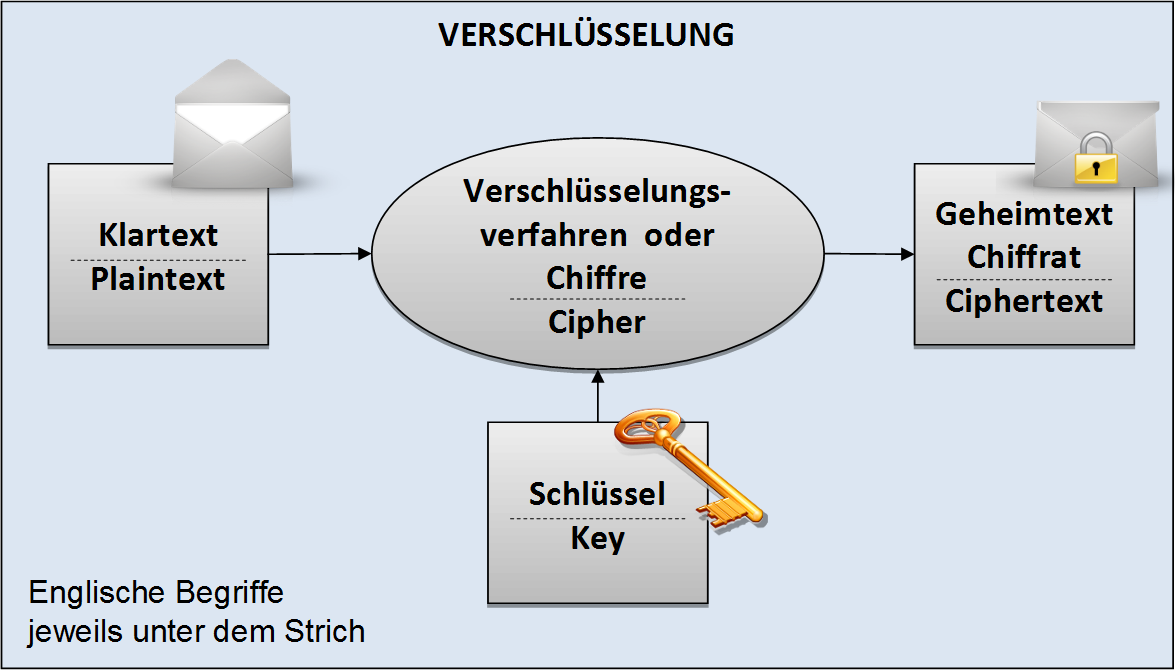
\includegraphics[scale=0.6]{figures/Generic-Notation-Encryption_de.png}
\caption{Übliche Bezeichnungen bei der Verwendung von Verschlüsselungsverfahren}
\label{cm_Generic-Notations-when-Encrypting}
\end{center}
\end{figure}



% --------------------------------------------------------------------------
\newpage

\begin{ctsquote}
Erkläre es mir, ich werde es vergessen.\\
Zeige es mir, ich werde es vielleicht behalten.\\
Lass es mich tun, und ich werde es können.
\caption{Indisches Sprichwort}
\end{ctsquote}


% --------------------------------------------------------------------------
\hypertarget{cm_Section_Security_Definitions}{}
\section{Sicherheits-Definitionen und Bedeutung der Kryptologie}
\label{cm_Section_Security_Definitions}
\index{Sicherheits-Definitionen}

Zuerst erklären wir, wie die Sicherheit von Kryptosystemen definiert wird.

Moderne Kryptographie basiert vor allem auf mathematischer Theorie und
Computer-Praxis. Beim Design kryptographischer Algorithmen werden Annahmen
zur Schwierigkeit von Berechnungen so gemacht, so dass sich solche Verfahren
in der Praxis von einem Angreifer nur schwer brechen lassen.

\vskip +3pt
Die zwei Hauptnotationen in der Literatur definieren Sicherheit in
Abhängigkeit von den Möglichkeiten des Angreifers (vgl. z.B.
{\em Contemporary Cryptography} \cite{Oppliger2011}):

\begin{itemize}

\item \textbf{Berechenbare, bedingte oder praktische Sicherheit}\\
  Ein Verschlüsselungsverfahren ist {\em berechenbar} sicher, wenn es (obwohl
  es theoretisch möglich ist, es zu brechen) selbst mit den besten bekannten
  Verfahren nicht gebrochen werden kann. Theoretische Fortschritte (z.B.
  Verbesserungen bei den Algorithmen zur Faktorisierung) und schnellere
  Computer erfordern, dass dies ständig angepasst wird.

  Selbst wenn man den besten bekannten Algorithmus zum Brechen benutzt, wird
  man so viele Ressourcen brauchen (z.B. 1.000.000 Jahre), dass das Kryptosystem
  sicher ist.

  Daher basiert dieses Konzept auf Annahmen über die begrenzte Rechenkraft des
  Angreifers und auf dem aktuellen Stand der Wissenschaft.

\item \textbf{Informations-theoretische oder unbedingte Sicherheit}\\
  Ein Verschlüsselungsverfahren wird als {\em unbedingt} sicher bezeichnet,
  wenn seine Sicherheit gewährleistet ist, völlig unabhängig davon, wieviele
  Ressourcen (Zeit, Speicher) der Angreifer hat -- also auch in dem Fall,
  wenn der Angreifer unbegrenzt viele Ressourcen hat, um das
  Verfahren zu brechen. Auch mit unbegrenzt vielen Ressourcen kann der
  Angreifer aus dem Chiffrat keine sinnvollen Informationen gewinnen.

  Es gibt Informations-theoretisch sichere Verfahren, die beweisbar nicht
  gebrochen werden können, auch nicht mit unendlich viel Rechenkraft -- ein
  Beispiel dafür ist das {\em One-Time-Pad} (OTP\index{OTP}).

  Da das OTP ein Informations-theoretisch sicheres Verschlüsselungsverfahren
  ist, leitet sich seine Sicherheit schon allein aus der Informationstheorie
  ab -- und ist sicher, auch wenn der Angreifer unbegrenzte Rechenkapazitäten
  hat. Das OTP weist allerdings einige praktische Nachteile auf (der
  verwendete Schlüssel darf nur einmal verwendet werden, muss zufällig
  gewählt werden und mindestens so lang sein wie die zu schützende Nachricht),
  so dass es außer in geschlossenen Umgebungen, zum Beispiel beim heißen
  Draht zwischen Moskau und Washington, kaum eine Rolle spielt.%\par \vskip + 3pt

\end{itemize}


\vskip +3pt
Manchmal werden auch zwei weitere Konzepte verwendet:

\begin{itemize}

\item \textbf{Beweisbare Sicherheit}
Dies bedeutet, dass das Brechen eines Kryptosystems mindestens so schwierig ist
wie die Lösung eines bestimmten schwierigen Problems, z.B. die Berechnung des
diskreten Logarithmus, die diskrete Quadratwurzel-Berechnung oder die
Faktorisierung sehr großer Zahlen.

Beispiel: Aktuell wissen wir, dass RSA\index{RSA} höchstens so schwierig
ist wie die Faktorisierung, aber wir können nicht beweisen, dass es genauso
schwierig ist.
Deshalb hat RSA keine beweisbare Mindest-Sicherheit. Oder in anderen Worten:
Wir können nicht beweisen, dass wenn das Kryptosystem RSA gebrochen ist, dass
dann auch die Faktorisierung (ein schwieriges mathematisches Problem) gelöst
werden kann.

Das Rabin-Kryptosystem war das erste Kryptosystem, für das sich beweisen ließ,
dass es berechenbar äquivalent zu einem harten mathematischen Problem ist.

\item \textbf{Ad-hoc-Sicherheit}
Ein kryptographisches System hat diese Sicherheit, wenn es sich nicht lohnt,
es zu versuchen es zu brechen, weil der Aufwand dafür teurer ist als der Wert
der Daten, die man durch das Brechen erhalten würde. Z.B. weil ein Angriff
nicht in einer ausreichend kurzen Zeit erfolgen kann (vgl.
{\em Handbook of Applied Cryptography} \cite{Menezes2001}).

Dies kann z.B. zutreffen, wenn Börsen-relevante Daten sowieso am
nächsten Tag veröffent"-licht werden und man für das Brechen ein Jahr brauchen
würde.

\end{itemize}


\vskip +3pt
Bei den heutzutage verwendeten guten Verfahren ist der Zeitaufwand zum Brechen
so hoch, dass sie praktisch nicht gebrochen werden können. Deshalb kann man
diese Verfahren als (praktisch) sicher ansehen -- aus einer rein auf den
Algorithmus bezogenen Sichtweise.\footnote{%
  Insbesondere seit den Informationen von Edward Snowden\index{Snowden, Edward} gab es
  viele Diskussionen, ob Verschlüsselung sicher ist. In \cite{Esslinger2014} wird das
  Ergebnis einer Evaluierung vorgestellt, auf welche Kryptographie man sich verlassen
  kann -- nach dem heutigen Kenntnisstand.
  Der Artikel untersucht: Welche Krypto-Verfahren können im Lichte der NSA-Enthüllungen
  noch als sicher gelten? Wo wurden Systeme gezielt geschwächt? Wie können wir die
  kryptographische Zukunft sicher gestalten? Wie unterscheiden sich Mathematik und
  Implementierung?
}

\vskip +3pt
\begin{sloppypar}
Grundsätz"-lich unterscheidet man zwischen symmetrischen
(siehe Kapitel \ref{cm_Section_Symmetric-encryption}) und asymmetrischen
(siehe Kapitel \ref{cm_Section_Asymmetric-encryption})
Verfahren zur Verschlüsse"-lung.
Einen sehr guten Überblick über die verschiedenen Verschlüsselungsverfahren
bieten auch die Bücher von Bruce Schneier \cite{Schneier1996} und Klaus Schmeh
\cite{Schm2016}.\footnote{%
  Einen kompakten Überblick, der erklärt, was wozu verwendet wird, welche der Verfahren
  sicher sind, wo mit Problemen zu rechnen ist und wo die wichtigen Baustellen für die
  absehbare Zukunft liegen incl. des Procederes bei den Standardisierungen finden Sie
  in \cite{Schmidt2016}.
  % TODO Info an ju, dass Schreibweise korr ("s" anhängen)
  %%     bei "Bereits 1883 formulierte Auguste Kerckhoff".
  % Dieser Artikel erschien ursprünglich in c't 01/2016, Seite 174
  % Kryptographie in der IT - Empfehlungen zu Verschlüsselung und Verfahren.
  % Kryptographie ist ein wichtiger Baustein moderner IT – Sicherheit,
  % Vertraulichkeit und Privatsphäre hängen davon ab. Der folgende Krypto-Wegweiser
  % gibt einen kompakten Überblick zu den aktuell relevanten Verfahren.
}
\end{sloppypar}

\vskip +3pt
Bevor Verschlüsselungstechnologien mit dem Aufkommen des Internets und der drahtlosen
Kommunikation für jedermann zur Verfügung standen, waren sie schon seit Jahrhunderten
im Gebrauch von Regierungen, Militärs und Diplomaten. Welche Seite diese Technologie
besser beherrschte konnte mit Hilfen der Geheimdienste großen Einfluss auf die \textbf{Politik}
und den Kriegsverlauf nehmen. Auf die Historie geht dieses Buch nur insofern ein, als
in Kapitel \ref{Chapter_PaperandPencil} auch die früher benutzten Verfahren vorgestellt
werden. Einen Eindruck, welch entscheidende Bedeutung Kryptologie für die Mächtigen
hatte und hat, kann man anhand der beiden folgenden Beispiele bekommen: dem Lehrfilm
\glqq Krieg der Buchstaben\grqq\footnote{%
  Der Film \index{Krieg der Buchstaben} schildert vor dem Hintergrund der Weltpolitik
  von 1900-1945 die Entwicklung der Kryptologie und ihre Bedeutung für den
  Kriegsverlauf im ersten (Zimmermann-Depesche) und zweiten Weltkrieg. Ausführlich
  wird -- aus anglo-amerikanischer Sicht -- darauf eingegangen, wie bedeutsam die
  Kryptoanalyse (auf dem Atlantik gegen die Enigma und auf dem Pazifik gegen Purple)
  für den Verlauf des zweiten Weltkriegs war.\\
  Siehe \url{https://bscw.schule.de/pub/bscw.cgi/d1269787/Krieg_der_Buchstaben.pdf}.
}
und der Debatte um die sogenannten Krypto-Wars\footnote{%
  Siehe \url{https://de.wikipedia.org/wiki/Crypto_Wars}.\index{Krypto-Wars}
}.
%% Vgl. http://scilogs.spektrum.de/hlf/verschluesselte-hintertuerchen-tag-internet-licht/
%%      http://www.heidelberg-laureate-forum.org/de/2015/08/17/eine-debatte-ueber-die-herausforderungen-einer-datengesteuerten-welt/
%%      http://wwwde.uni.lu/snt/news_events/prof_peter_ryan_gives_lecture_at_heidelberg_laureate_forum
%% Diskussion auf dem 3. Heidelberg Laureate Forum (HLF) am Dienstag, 25. August 2015.


% --------------------------------------------------------------------------
\newpage

\begin{ctsquote}
\glqq Man kann nicht nicht kommunizieren!\grqq
\caption[Paul Watzlawick]{Paul Watzlawick\footnotemark}\index{Watzlawick, Paul}
\end{ctsquote}
\addtocounter{footnote}{0}\footnotetext{Paul Watzlawick, Janet H. Beavin und Don D. Jackson, \glqq Menschliche Kommunikation. Formen, Störungen, Paradoxien\grqq, Huber, (c) 2007, Das erste der fünf pragmatischen Axiome ihrer Kommunikationstheorie.}

% --------------------------------------------------------------------------
\section[Einflüsse auf Verschlüsselungsverfahren] % Was zw. [..] steht, kommt ins Inhaltsverzeichnis!
{Einflüsse auf Verschlüsselungsverfahren}

% \nopagebreak
Hier sollen kurz zwei Aspekte von Kryptoverfahren erwähnt werden, auf die oft nicht früh genug eingegangen wird:

\begin{itemize}

\item \textbf{Zufallsbasiert}\\
\index{Zufall}
Man kann Algorithmen aufteilen in deterministische\index{deterministisch} und heuristische\index{heuristisch} Verfahren. Meistens lernten Studenten nur deterministische Verfahren kennen, bei denen die Ausgabe eindeutig durch die Eingabe vorgegeben wird. Bei heuristischen Verfahren werden Entscheidungen aufgrund zufälliger Werte getroffen. Moderne Verfahren des maschinellen Lernens gehören ebenfalls hierzu.

In Kryptoverfahren spielt Zufall eine große Rolle. Immer müssen die Schlüssel zufällig gewählt werden, so dass zumindest bei der Schlüsselgenerierung~\glqq Zufall\grqq~erzeugt werden muss. Zusätzlich sind manche Verfahren (vor allem aus der Kryptoanalyse) heuristisch.

\item \textbf{Konstanten-basiert}\\
Viele moderne Verfahren (insbesondere Hashverfahren und symmetrische Verschlüsse-lungsverfahren) benutzen numerische Konstanten. Diese sollten nachvollziehbar sein und keine Hintertüren ermöglichen. Zahlen, die das erfüllen, nennt man im Englischen~\glqq Nichts-im-Ärmel\grqq-Zahlen: Nothing-up-my-sleeve number\index{Zahlen!Nothing-up-my-sleeve}.%
\footnote{\url{http://en.wikipedia.org/wiki/Nothing_up_my_sleeve_number}}

\end{itemize}


\newpage
Die folgende Abbildung \ref{cm_Figure_OTP-demo-pictures} soll eine Idee davon vermitteln, dass es nicht möglich ist, bei einem OTP\index{OTP} den Klartext zu bestimmen (sofern das OTP-Verfahren richtig angewendet wird und alle Schlüssel gleich wahrscheinlich sind).

In dem Beispiel in der Abbildung ist als Geheimtext ein 8 Zeichen langes Wort gegeben:
\texttt{11 1B 1E 18 00 04 0A 15}.
Es gibt viele sinnvolle Worte aus 8 Buchstaben und zu jedem einen passenden Schlüssel.
Ein Angreifer kann damit allein nicht bestimmen, welches der richtige Schlüssel bzw.
welches das richtige Klartext-Wort ist.

Vergleiche auch Abbildung~\ref{fig-bool-otp} in Kapitel \ref{s-bool-bitstr-real-random},
wo ein entsprechendes Text-Beispiel mit SageMath erstellt wird.
\begin{figure}[ht]
\begin{center}
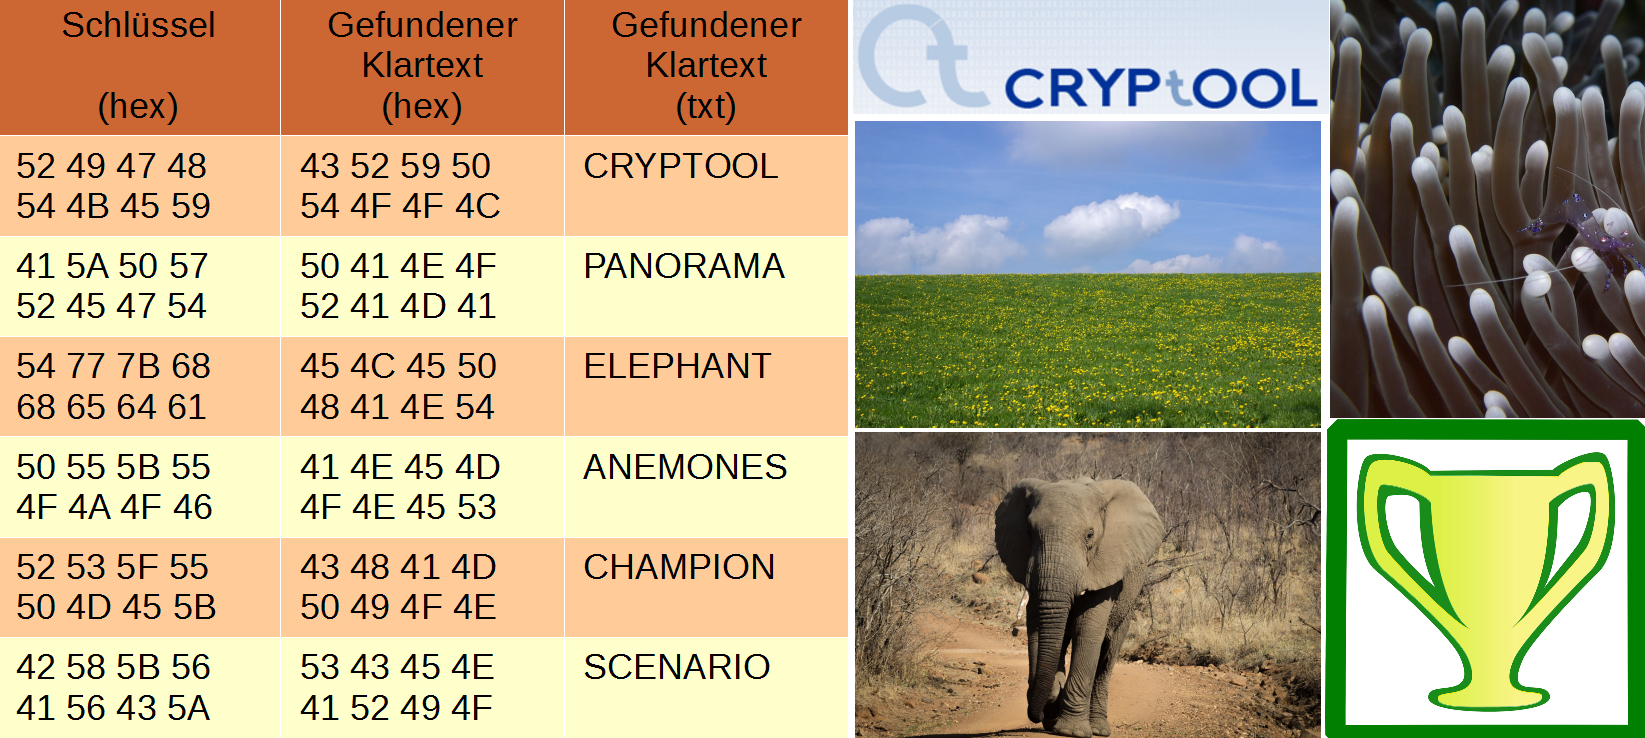
\includegraphics[scale=0.54]{figures/OTP-demo-pictures-de.png}
\caption[Illustration für die Informations-theoretische Sicherheit des OTP]
        {Illustration für die Informations-theoretische Sicherheit des OTP\footnotemark}
\label{cm_Figure_OTP-demo-pictures}
\end{center}
\end{figure}
\footnotetext{
  Bildquelle: Kostenlose Bilder von \url{https://pixabay.com/}
}





% --------------------------------------------------------------------------
\newpage

\begin{ctsquote}
\glqq Transparenz. Das ist das Höchste, was man sich in einer technologisch hoch entwickelten Gesellschaft erhoffen kann ... sonst wird man einfach nur manipuliert.\grqq
\caption[Daniel Suarez]{Daniel Suarez\footnotemark}\index{Suarez, Daniel}
\end{ctsquote}
\addtocounter{footnote}{0}\footnotetext{Daniel Suarez, \glqq Darknet\grqq,
            rororo, (c) 2011, Kapitel 5, \glqq Einsichten\grqq, S. 69, Price.}

% --------------------------------------------------------------------------
\section[Symmetrische Verschlüsselung] % Was zwischen [...] steht, kommt ins Inhaltsverzeichnis!
        {Symmetrische Verschlüsselung\footnotemark}
  \footnotetext{% Dieses Prozent ist nötig, sonst startet die Fußnote mit einem Blank !
    Mit CrypTool~1 (\textbf{CT1})\index{CT1} können Sie über das
    Menü \textbf{Ver-/Entschlüsseln \textbackslash{} Symmetrisch (modern)} folgende
    modernen symmetrischen Verschlüsselungsverfahren ausführen:\\
    IDEA, RC2, RC4, DES (ECB), DES (CBC), Triple-DES (ECB), Triple-DES (CBC),
    MARS (AES-Kandidat), RC6 (AES-Kandidat), Serpent (AES-Kandidat),
    Twofish (AES-Kandidat),
    Rijndael (offizielles AES-Verfahren)\index{AES}.\\
    Mit CrypTool~2 (\textbf{CT2})\index{CT2} können Sie im Startcenter
    über \textbf{Vorlagen \textbackslash{} Kryptographie \textbackslash{}
    Modern \textbackslash{} Symmetrisch} folgende modernen symmetrischen
    Verschlüsselungsverfahren ausführen:\\
    AES, DES, PRESENT, RC2, RC4, SDES, TEA, Triple-DES, Twofish.\\
    In JCrypTool (\textbf{JCT})\index{JCT} stehen Ihnen die folgenden
    modernen symmetrischen Verschlüsselungsverfahren zur Verfügung:\\
    AES, Rijndael, Camellia, DES, Dragon, IDEA, LFSR, MARS, Misty1, RC2, RC5,
    RC6, SAFER+, SAFER++, Serpent, Shacal, Shacal2, Twofish.
    }
\label{cm_Section_Symmetric-encryption}

\nopagebreak

Bei der {\em symmetrischen} Verschlüsselung
\index{Verschlüsselung!symmetrisch} müssen Sender und Empfänger
über einen gemeinsamen (geheimen) Schlüssel verfügen, den sie vor
Beginn der eigentlichen Kommunikation ausgetauscht haben. Der Sender
benutzt diesen Schlüssel, um die Nachricht zu verschlüsseln und der
Empfänger, um diese zu entschlüsseln.\par %\vskip + 3pt

Dies veranschaulicht Abbildung \ref{cm_Figure_Symmetric-Enc_Secret-Key-Enc}:
\begin{figure}[ht]
\begin{center}
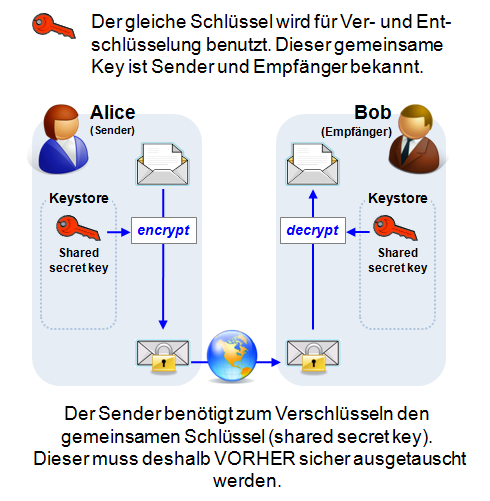
\includegraphics[scale=0.7]{figures/SymmetricEnc_Figure_Chap1_de.png}
\caption{Symmetrische oder Secret-Key-Verschlüsselung}
\label{cm_Figure_Symmetric-Enc_Secret-Key-Enc}
\end{center}
\end{figure}

Alle klassischen Chiffren sind vom Typ symmetrisch. Beispiele dazu finden Sie
in den CT-Programmen, im Kapitel~\ref{Chapter_PaperandPencil}
(\glqq \nameref{Chapter_PaperandPencil}\grqq)
in diesem Skript oder in \cite{Nichols1996}.
In diesem Unterkapitel wollen wir jedoch nur die moderneren symmetrischen
Verfahren betrachten.

Vorteile von symmetrischen Algorithmen sind die hohe
Geschwindigkeit, mit denen Daten ver- und entschlüsselt werden.
Ein Nachteil ist das Schlüsselmanagement. Um miteinander
vertraulich kommunizieren zu können, müssen Sender und
Empfänger vor Beginn der eigentlichen Kommunikation über einen
sicheren Kanal einen Schlüssel ausgetauscht haben. Spontane
Kommunikation zwischen Personen, die sich vorher noch nie begegnet
sind, scheint so nahezu unmöglich. Soll in einem Netz mit $ n $
Teilnehmern jeder mit jedem zu jeder Zeit spontan kommunizieren
können, so muss jeder Teilnehmer vorher mit jedem anderen der
$n - 1$ Teilnehmer einen Schlüssel ausgetauscht haben. Insgesamt
müssen also $n(n - 1)/2$ Schlüssel ausgetauscht werden.\par \vskip + 3pt



\subsection[AES (Advanced Encryption Standard)]{AES (Advanced Encryption Standard)\footnotemark}
\footnotetext{%
   In CT1\index{CT1} finden Sie 3 Visualisierungen dieses Verfahrens
   über das Menü \textbf{Einzelverfahren \textbackslash{} Visualisierung von
   Algorithmen \textbackslash{} AES}.\\
   In CT2\index{CT2} können Sie im Startcenter
   mit dem Suchstring \glqq AES\grqq~eine Vorlage (Template) finden,
   die den Algorithmus Schritt-für-Schritt visualisiert.
}
\label{CM_AES}
\index{AES}

Vor AES war der DES-Algorithmus\index{DES} das bekannteste moderne, symmetrische
Verschlüsselungs"-ver"-fahren. Der DES-Algorithmus war eine Entwicklung von IBM
in Zusammenarbeit mit der National Security Agency \index{NSA} (NSA).
Er wurde 1975 als Standard veröffentlicht. Trotz seines relativ hohen
Alters ist bis heute kein~\glqq effektiver\grqq~Angriff auf
ihn gefunden worden. Der effektivste Angriff besteht aus dem Durchprobieren
(fast) aller möglichen Schlüssel, bis der richtige gefunden wird
({\em Brute-Force-Angriff})\index{Angriff!Brute-Force}. Aufgrund der relativ
kurzen Schlüssellänge von effektiv 56 Bits (64 Bits, die allerdings 8
Paritätsbits enthalten), sind in der Vergangenheit schon mehrfach mit dem
DES verschlüsselte Nachrichten gebrochen worden, so dass er heute nicht
mehr als sicher anzusehen ist. Alternativen zum DES sind zum Beispiel die
Algorithmen IDEA\index{IDEA}, Triple-DES (TDES) und vor allem AES.
\par \vskip + 3pt

Standard unter den symmetrischen Verfahren ist heute AES\index{AES}:
Der dazu gehörende Rijndael-Algo"-rithmus wurde am 2. Oktober 2000 zum
Gewinner der AES-Ausschreibung erklärt und ist damit Nachfolger
des DES-Verfahrens.

Einen Einstieg und weitere Verweise zum AES-Algorithmus und den AES-Kandidaten
der letzten Runde finden Sie z.B. in der Online-Hilfe von
CrypTool\index{CrypTool}%
\footnote{%
      Online-Hilfe von CT1\index{CT1}: Das Stichwort \textbf{AES} im Index
      führt auf die drei Hilfeseiten: \textbf{AES-Kandidaten},
      \textbf{Der AES-Gewinner Rijndael} und \textbf{Der AES-Algorithmus Rijndael}.\\
      Eine ausführliche Beschreibung von AES mit C-Code findet sich
      in \cite{Haan2008}.
  }
oder in Wikipedia%
\footnote{%
	\url{https://de.wikipedia.org/wiki/Advanced_Encryption_Standard}
  }.


\clearpage
Die beiden Screenshots \ref{AES-Visualization-Zabala-Flash-step3} und
\ref{AES-Visualization-Zabala-Flash-step5} sind aus einer der 3
AES-Visualisierungen in CT1\index{CT1}.

% Ohne das !vor ht verteilt LaTeX die abb. auf 2 Seiten. \sloppypar hilft hier nict (nur für Worttrenner).
% http://texwelt.de/wissen/fragen/6667/mehrere-bilder-untereinander
\begin{figure}[!ht]
\begin{center}
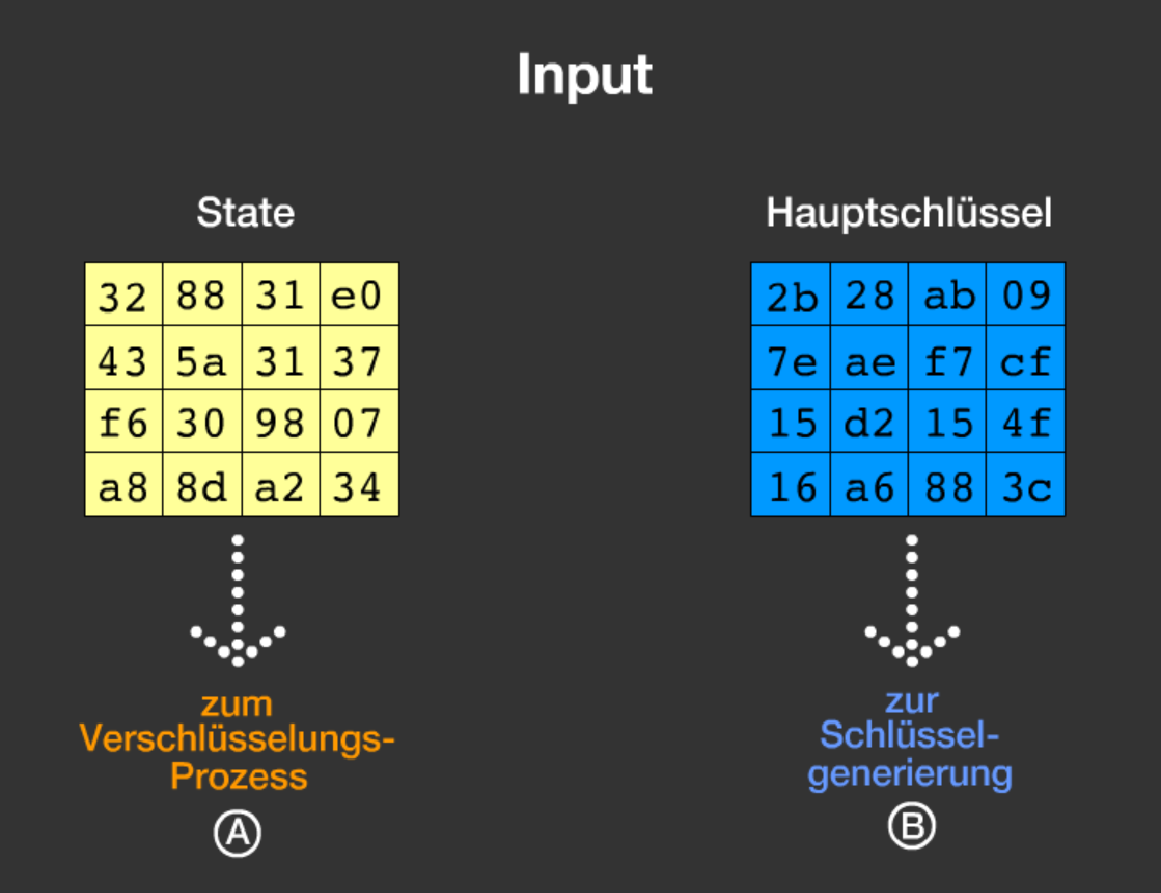
\includegraphics[scale=0.6]{figures/AES-Visualization-Zabala-Flash-step3_de}
\caption{AES-Visualisierung von Enrique Zabala aus CT1 (Teil 1)}
\label{AES-Visualization-Zabala-Flash-step3}
\end{center}
\end{figure}

\begin{figure}[!ht]
\begin{center}
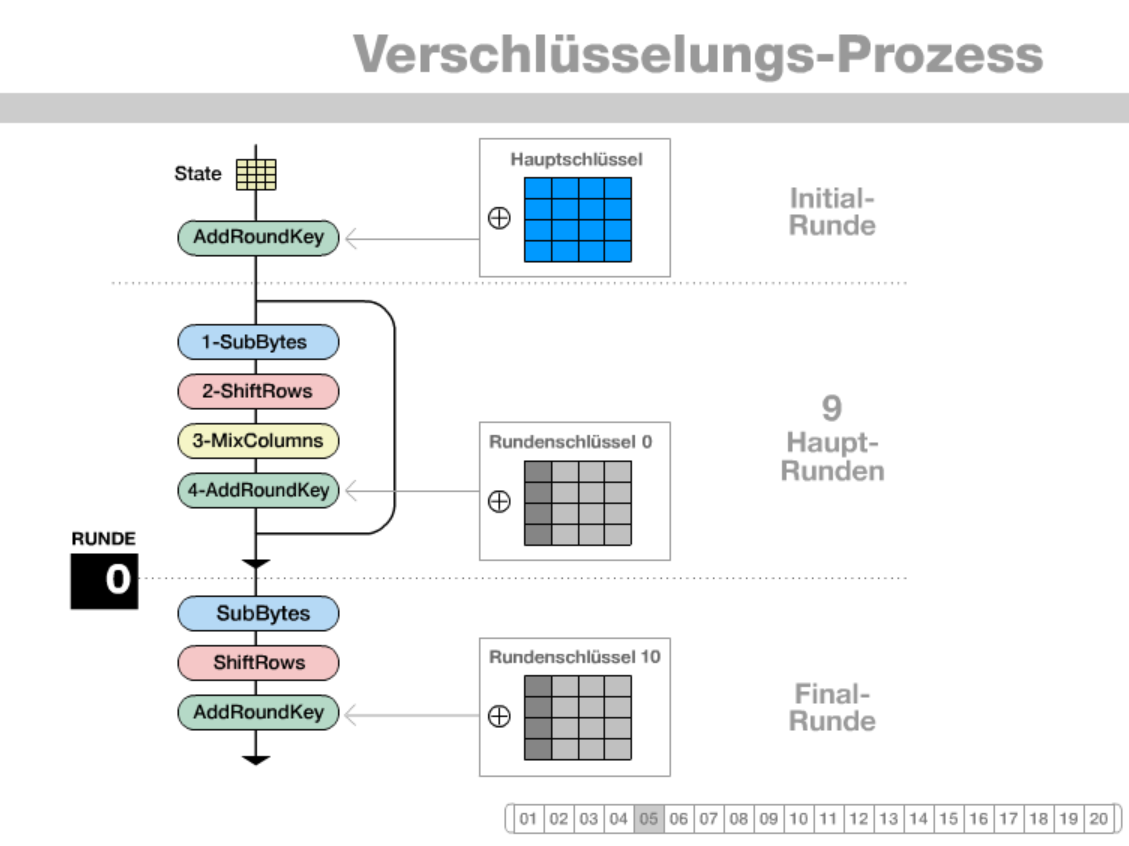
\includegraphics[scale=0.6]{figures/AES-Visualization-Zabala-Flash-step5_de}
\caption{AES-Visualisierung von Enrique Zabala aus CT1 (Teil 2)}
\label{AES-Visualization-Zabala-Flash-step5}
\end{center}
\end{figure}
%\end{sloppypar}


\clearpage
Im Folgenden wollen wir einen 128-bit-Block Klartext mit einem 128-bit
Schlüssel mit AES im CBC-Modus verschlüsseln. Vom erhaltenen Geheimtext interessiert
uns nur der 1. Block (wenn mehr vorhanden ist, ist das Padding -- hier Null-Padding).
Zur Veranschaulichung machen wir das einmal mit CT2 und einmal mit OpenSSL.\\

Abbildung \ref{AES_Encrypting-one-block-with-CT2} zeigt die Verschlüsselung
eines Blocks in \textbf{CT2}\index{CT2}.

Der Klartext \glqq AESTEST1USINGCT2\grqq~wird nach Hex
(41 45 53 54 45 53 54 31 55 53 49 4E 47 43 54 32)
konvertiert. Damit und mit dem Schlüssel 3243F6A8885A308D313198A2E0370734
erzeugt die AES-Komponente dann den Geheimtext. Dieser lautet in Hex:\\
B1 13 D6 47 DB 75 C6 D8 47 FD 8B 92 9A 29 DE 08

\begin{figure}[ht]
\begin{center}
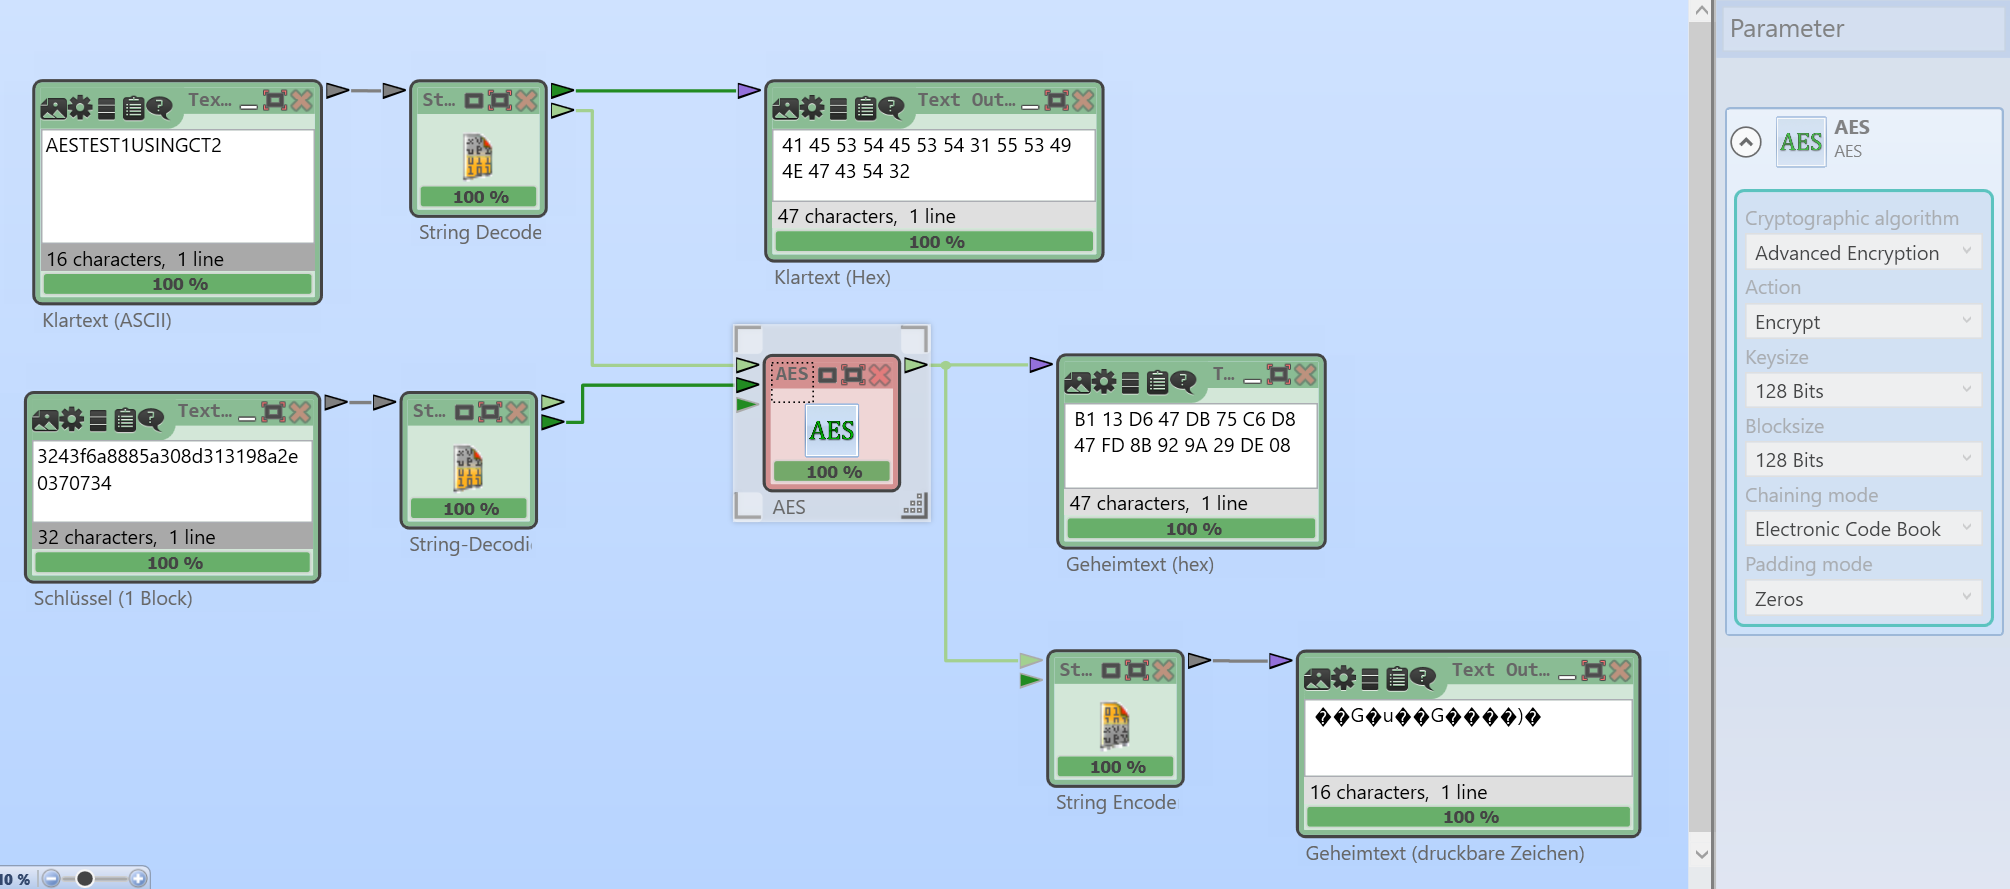
\includegraphics[scale=0.42]{figures/AES_Encrypting-one-block-with-CT2_de}
\caption{AES-Verschlüsselung (genau 1 Block ohne Padding) in CT2}
\label{AES_Encrypting-one-block-with-CT2}
\end{center}
\end{figure}

\vspace{15pt}
Dasselbe Ergebnis kann man mit \textbf{OpenSSL}\index{OpenSSL}%
\footnote{%
      OpenSSL\index{OpenSSL} ist eine sehr verbreitete freie Open-Source Kryptobibliothek,
      die von vielen Anwendungen benutzt wird, bspw. um das TLS-Protokoll zu implementieren.
      Zu OpenSSL gehört auch das Kommandozeilentool openssl, mit dem man die Funktionalität
      auf vielen Betriebssystemen direkt ausprobieren und Zertifikate beantragen, erzeugen
      und verwalten kann.\\
      Im Gegensatz zum ebenfalls sehr verbreiteten und sehr guten Kommandozeilentool gpg
      von GNU Privacy Guard\index{GnuPG}
      (\url{https://de.wikipedia.org/wiki/GNU_Privacy_Guard})
      erlaubt openssl auch Aufrufe, die sehr ins Detail gehen.
      Bei gpg liegt der Schwerpunkt auf den im praktischen Einsatz befindlichen Ciphersuites.
      Einfach genau einen Block ohne Padding zu verschlüsseln geht unseres Wissens mit dem
      Kommandozeilentool gpg nicht.\\
      Siehe auch \url{https://de.wikipedia.org/wiki/OpenSSL}.
%      Also see \url{https://en.wikipedia.org/wiki/OpenSSL}.
  }
auf der Kommandozeile auf ff. Weise erzielen:
\begin{opensslcode}
\begin{Verbatim}%
[fontsize=\footnotesize]
>openssl enc -e -aes-128-cbc
        -K 3243F6A8885A308D313198A2E0370734
        -iv 00000000000000000000000000000000
        -in klartext-1.hex  -out klartext-1.hex.enc
>dir
06.07.2016  12:43                16 key.hex
20.07.2016  20:19                16 klartext-1.hex
20.07.2016  20:37                32 klartext-1.hex.enc
\end{Verbatim}
\caption{AES-Verschlüsselung (von genau einem Block ohne Padding) in OpenSSL}
\label{cm_AES_no-padding:OpenSSL_example}
\end{opensslcode}





\clearpage
% HACK to fix warning "destination with the same identifier .. has already been used, ...":
% REMOVED, because it caused missing index entries
%\makeatletter \renewcommand{\thepage}{\csname @arabic\endcsname \c@page} \makeatother
% --------------------------------------------------------------------------
\subsubsection{Ergebnisse zur theoretischen Kryptoanalyse von AES}
\label{cm_New-AES-Analysis}
\index{Kryptoanalyse}
\index{AES}

Im Anschluss finden Sie einige Informationen, die das AES-Verfahren in
letzter Zeit in Zweifel zogen -- unserer Ansicht nach aber (noch)
unbegründet. Die folgenden Informationen beruhen vor allem auf den unten
angegebenen Originalarbeiten und auf \cite{Wobst2002} und
\cite{Lucks2002}.

Der AES bietet mit einer Mindestschlüssellänge von 128 Bit gegen
Brute-Force-Angriffe auch auf längere Sicht genügend Sicherheit -- es sei
denn, es stünden entsprechend leistungsfähige Quantencomputer zur
Verfügung. Der AES war immun gegen alle bis dahin bekannten
Krypto"-analyse-Verfahren, die vor allem auf statistischen
Überlegungen beruhen und auf DES angewandt wurden: man konstruiert aus
Geheim- und Klartextpaaren Ausdrücke, die sich nicht rein zufällig
verhalten, sondern Rückschlüsse auf den verwendeten Schlüssel zulassen.
Dazu waren aber unrealistische Mengen an abgehörten Daten nötig.

Bei Kryptoverfahren bezeichnet man solche Kryptoanalyseverfahren als
"`akademischen Erfolg"' oder als "`kryptoanalytischen Angriff"', da sie
theoretisch schneller sind als das Durchprobieren aller Schlüssel, das
beim Brute-Force-Angriff\index{Angriff!Brute-Force} verwendet wird. Im
Fall des AES mit maximaler Schlüssellänge (256 Bit) braucht die
erschöpfende Schlüsselsuche im Durchschnitt $2^{255}$
Verschlüsselungsoperationen. Ein kryptoanalytischer Angriff muss diesen
Wert unterbieten. Als aktuell gerade noch praktikabel (z.B. für einen
Geheimdienst) gilt ein Aufwand von $2^{75}$ bis $2^{90}$
Verschlüsselungsoperationen.

Eine neue Vorgehensweise wurde in der Arbeit von Ferguson, Schroeppel
und Whiting im Jahre 2001 \cite{Ferguson2001} beschrieben: Sie stellten
AES als geschlossene Formel (in der Form einer Art Kettenbruch) dar,
was aufgrund seiner "`relativ"' übersichtlichen Struktur gelang. Da
diese Formel aus rund 1 Billiarde Summanden besteht, taugt sie zunächst
nicht für die Kryptoanalyse. Dennoch war die wissenschaftliche Neugier
geweckt. Bereits bekannt war, dass sich der 128-Bit-AES als ein
überbestimmtes System von rund 8000 quadratischen Gleichungen
(über algebraischen Zahlkörpern) mit rund 1600 Variablen (einige
Unbekannte sind die Schlüsselbits) darstellen lässt -- solch große
Gleichungssysteme sind praktisch nicht lösbar. Dieses Gleichungssystem
ist relativ dünn besetzt (\glqq sparse\grqq), d.h. von den insgesamt etwa
1.280.000 möglichen quadratischen Termen tauchen nur relativ wenige
überhaupt im Gleichungssystem auf.

Die Mathematiker Courtois und Pieprzyk \cite{Courtois2002} veröffentlichten
2002 eine Arbeit, die in der Krypto-Szene stark diskutiert wird: Sie
entwickelten das auf der Eurocrypt 2000 von Shamir et al. vorgestellte
XL-Verfahren (eXtended Linearization) weiter zum XSL-Verfahren
(eXtended Sparse Linearization). Das XL-Verfahren ist eine heuristische
Technik, mit der es manchmal gelingt, große nicht-lineare Gleichungssysteme
zu lösen und die bei der Analyse eines asymmetrischen Algorithmus (HFE)
angewandt wurde.  Die Innovation von Courtois und Pieprzyk war, das
XL-Verfahren auf symmetrische Verfahren anzuwenden: Das XSL-Verfahren kann
auf spezielle Gleichungssysteme angewandt werden. Damit könnte ein
256-Bit-AES-Verfah"-ren in rund $2^{230}$ Schritten geknackt werden. Dies ist
zwar immer noch ein rein akademischer Angriff, aber er ist richtungsweisend
für eine ganze Klasse von Blockchiffren. Das generelle Problem mit diesem
Angriff besteht darin, dass man bisher nicht angeben kann, unter welchen
Umständen er zum Erfolg führt: die Autoren geben in ihrer Arbeit notwendige
Bedingungen an; es ist nicht bekannt, welche Bedingungen hinreichend sind.
Neu an diesem Angriff war erstens, dass dieser Angriff nicht auf Statistik,
sondern auf Algebra beruhte. Dadurch erscheinen Angriffe möglich, die nur
geringe Mengen von Geheimtext brauchen. Zweitens steigt damit die Sicherheit
eines Produktalgorithmus%
\index{Produktalgorithmus}\index{Verschlüsselung!Produktalgorithmus}%
\footnote{%
Ein Geheimtext kann selbst wieder Eingabe für eine Chiffrierung sein. Eine
Mehrfachverschlüsselung (cascade cipher)
\index{Verschlüsselung!Mehrfachverschlüsselung}\index{Mehrfachverschlüsselung}
\index{Kaskaden}
entsteht aus einer Komposition von mehreren Verschlüsselungstransformationen.
Die Gesamtchiffrierung wird Produktalgorithmus oder Kaskadenalgorithmus
genannt (manchmal ist die Namensgebung abhängig davon, ob die verwendeten
Schlüssel statistisch abhängig oder unabhängig sind).\\
Nicht immer wird die Sicherheit eines Verfahrens durch Produktbildung
erhöht.\\
Dieses Vorgehen wird auch {\em innerhalb} moderner Algorithmen angewandt:
Sie kombinieren in der Regel einfache und, für sich genommen, kryptologisch
relativ unsichere Einzelschritte in mehreren Runden zu einem leistungsfähigen
Gesamtverfahren. Die meisten modernen Blockchiffrierungen (z.B. DES, IDEA)
sind Produktalgorithmen.\\
Als Mehrfachverschlüsselung wird auch das Hintereinanderschalten desselben
Verfahrens mit verschiedenen Schlüsseln wie bei Triple-DES bezeichnet.\index{DES!Triple-DES}
}
nicht mehr exponentiell mit der Rundenzahl.

Aktuell wird sehr intensiv auf diesem Gebiet geforscht: z.B. stellten
Murphy und Robshaw auf der Crypto 2002 ein Papier vor \cite{Robshaw2002a},
das die Kryptoanalyse drastisch verbessern könnte: Der Aufwand für
128-Bit-Schlüssel wurde auf $2^{100}$ geschätzt, indem sie AES als
Spezialfall eines Algorithmus BES (Big Encryption System) darstellten,
der eine besonders "`runde"' Struktur hat. Aber auch $2^{100}$
Rechenschritte liegen jenseits dessen, was praktisch in absehbarer Zeit
realisierbar ist. Bei 256 Bit Schlüssellänge schätzen die Autoren
den Aufwand für den XSL-Angriff auf $2^{200}$ Operationen.

Weitere Details finden Sie unter den Weblinks bei
\hyperlink{CM_HT_Weblink_Rijndael-Cryptosystem}{\glqq Das AES-/Rijndael-Kryptosystem\grqq}.
% nur \href oder \url rückt nicht ein, deshalb \item dazu !
%\vspace{-10pt}
%\begin{itemize}
%  \item[] \url{http://www.cryptosystem.net/aes} \\
%          \url{http://www.minrank.org/aes/}
%\end{itemize}


Für AES-256 wäre der Angriff ebenfalls viel besser als
Brute-Force\index{Angriff!Brute-Force}, aber noch weit außerhalb der
Reichweite realisierbarer Rechenpower.

\begin{sloppypar}
Die Diskussion war zeitweise sehr kontrovers: Don Coppersmith (einer der
DES-Erfinder) z.B. bezweifelte die generelle Durchführbarkeit des Angriffs:
XLS liefere für AES gar keine Lösung \cite{Coppersmith2002}. Dann würde
auch die Optimierung von Murphy und Robshaw \cite{Robshaw2002b} nicht
greifen.
\end{sloppypar}

2009 veröffentlichten Biryukov und Khovratovich \cite{Biryukov2009} einen
weiteren theoretischen Angriff auf AES, der sich anderer Techniken bedient, als
die oben vorgestellten. Sie verwenden Methoden aus der Kryptoanalyse von
Hashfunktionen (lokale Kollisionen und das Boomerang-Verfahren) und
konstruierten daraus einen Related-Key-Angriff auf AES-256. D.~h.\ der Angreifer
muss nicht nur in der Lage sein, beliebige Daten zu verschlüsseln (chosen plain
text), sondern auch den ihm unbekannten Schlüssel manipulieren können (related
key).

Unter diesen Angriffs-Voraussetzungen reduziert der Angriff den Aufwand, einen
AES-256-Schlüssel zu ermitteln, auf eine (asymmetrische) Komplexität von
$2^{119}$ Zeit und $2^{77}$ Speicher. Bei AES-192 ist der Angriff noch weniger
praktikabel, für AES-128 geben die Autoren keinen Angriff an.


% --------------------------------------------------------------------------
\subsection{Algebraische oder algorithmische Kryptoanalyse symmetrischer Verfahren}
\index{Angriff!algebraisch}
\label{cm_Algebraic-versus-Symmetr}

Es gibt unterschiedliche moderne Angriffsverfahren, die die Strukturen eines Problems direkt oder nach einer Transformation des Problems angreifen. Eines dieser Angriffsverfahren beruht auf dem Erfüllbarkeitsproblem der Aussagenlogik (SAT, von englisch satisfiability)%
\footnote{%
 \url{http://de.wikipedia.org/wiki/Erf%C3%BCllbarkeitsproblem_der_Aussagenlogik}
}.


%\vskip +25 pt
\paragraph*{Beschreibung SAT-Solver}\index{SAT-Solver}\mbox{}
\hypertarget{ht_SAT-Solver}{}

Ein sehr altes und gut studiertes Problem in der Informatik ist das sogenannte SAT-Problem. Hier gilt es, für eine gegebene Boolesche Formel herauszufinden, ob es eine Belegung der Variablen gibt, so dass die Auswertung der Formel den Wert 1 ergibt.

Beispiel: Die Formel \glqq A UND B\grqq~wird zu 1 ausgewertet, wenn A=B=1 gilt. Für die Formel \glqq A UND NICHT(A)\grqq~gibt es keine Belegung für A, so dass sie zu 1 ausgewertet wird.

Für größere Formeln ist es nicht so einfach herauszufinden, ob eine Formel zu 1 ausgewertet werden kann (dieses Problem gehört zu den NP-vollständigen Problemen). Daher wurden spezielle Tools entwickelt, um dieses Problem für generelle Boolesche Formeln zu lösen, sogenannte SAT-Solver\footnote{
    Mit \textbf{CT2}\index{CT2} können Sie im Startcenter
    über \textbf{Vorlagen \textbackslash{} Mathematisch \textbackslash{}
    SAT-Solver (Texteingabe)}  und  \textbf{SAT-Solver (Dateieingabe)} einen
    SAT-Solver aufrufen.
    }. Wie sich herausgestellt hat, können SAT-Solver auch eingesetzt werden, um Krypto-Verfahren
anzugreifen.


%\vskip +25 pt
\paragraph*{SAT-Solver basierte Kryptoanalyse}\index{SAT-Solver}\mbox{}
\hypertarget{ht_SAT-Solver_Cryptanalysis}{}

Der generelle Ansatz, um SAT-Solver in der Kryptoanalyse einzusetzen, ist sehr einfach: Zunächst wird das kryptographische Problem, etwa das Finden des symmetrischen Schlüssels oder die Umkehrung einer Hashfunktion, in ein SAT-Problem übersetzt. Dann wird ein SAT-Solver verwendet, um eine Lösung für das SAT-Problem zu finden. Die Lösung des SAT-Problems löst dann auch das ursprüngliche kryptographische Problem.
Der Artikel von Massacci \cite{Massacci2000} beschreibt die erste bekannte Verwendung eines SAT-Solvers in diesem Kontext. Leider stellte sich sehr bald heraus, dass ein solch genereller Ansatz in der Praxis nicht effizient eingesetzt werden kann. Die kryptographischen SAT-Probleme sind sehr komplex und die Laufzeit eines SAT-Solvers wächst exponentiell mit der Problemgröße. Daher werden in modernen Ansätzen SAT-Solver nur für das Lösen von Teilproblemen der Kryptoanalyse verwendet. Ein gutes Beispiel zeigt der Artikel von Mironov und Zhang \cite{Mironov2006}. Hier wird anhand eines Angriffs auf Hashfunktionen gezeigt, zur Lösung welcher Teilprobleme SAT-Solver effizient eingesetzt werden können.

% Todo later: xxxxxxxxx Bsp aus CT2.1 ergänzen mit SAT-Analyzer (nicht nur SAT-Solver)
%             Erfordert wahrscheinlich den CT2-Store, da es vorerst nur mit cygwin läuft.
% \index{ZZZ6b-xxxxxxxxxxxxxxxx-Bsp aus CT2.1 ergaenzen}
% \index{ZZZ6b-xxxxxxxxxxxxxxxxD}




% --------------------------------------------------------------------------
\subsection{Aktueller Stand der Brute-Force-Angriffe auf symmetrische Verfahren}
\index{Angriff!Brute-Force}
\index{RC5}
\label{cm_Brute-force-versus-Symmetr}

Anhand der Blockchiffre RC5 kann der aktuelle Stand von Brute-Force-Angriffen
auf symmetrische Verschlüsselungsverfahren gut erläutert werden.

\begin{sloppypar}
Als Brute-Force-Angriff (exhaustive search, trial-and-error) bezeichnet
man das vollständige Durchsuchen des Schlüsselraums: Dazu müssen
keine besonderen Analysetechniken eingesetzt werden. Stattdessen wird
der Geheimtext mit allen möglichen Schlüsseln des Schlüsselraums
entschlüsselt%
\footnote{%
  Mit CT1\index{CT1} können Sie über das Menü
  \textbf{Analyse \textbackslash{} Symmetrische Verschlüsselung (modern)}
  ebenfalls Brute-Force-Analysen von modernen symmetrischen Verfahren
  durchführen (unter der schwächsten aller möglichen Annahmen: Der
  Angreifer kennt nur den Geheimtext, er führt also einen
  Ciphertext-only-Angriff durch).\\
  Mit CT2\index{CT2} können Sie bei den Vorlagen unter
  \textbf{Kryptoanalyse \textbackslash{} Modern} ebenfalls Brute-Force-Analysen
  durchführen. Besonders mächtig ist die KeySearcher-Komponente, die
  die Ausführung auch auf mehrere Rechner verteilen kann.
}
und geprüft, ob der resultierende Text einen sinnvollen
Klartext ergibt%
\footnote{%
  Ist der Klartext natürlich-sprachlich und wenigstens 100 B lang, kann
  diese Prüfung ebenfalls automatisiert durchgeführt werden.\\
  Um in einer sinnvollen Zeit auf einem Einzel-PC ein Ergebnis zu
  erhalten, sollten Sie nicht mehr als 24 Bit des Schlüssels als
  unbekannt kennzeichnen.}.
Bei einer Schlüssellänge von 64 Bit sind dies maximal
$2^{64}$ = 18.446.744.073.709.551.616 oder rund 18 Trillionen zu
überprüfende Schlüssel\index{CrypTool}.
\end{sloppypar}

Um zu zeigen, welche Sicherheit bekannte symmetrische Verfahren wie
DES, Triple-DES oder RC5\index{DES}\index{RC5}\index{DES!Triple-DES}
haben, veranstaltete z.B. RSA Security
sogenannte Cipher-Challenges\index{Challenge}.\footnote{%
  \url{https://www.emc.com/emc-plus/rsa-labs/historical/the-rsa-laboratories-secret-key-challenge.htm}\\
  Im Mai 2007 meldete RSA Inc leider, dass sie die Korrektheit der bis dahin
  nicht gelösten RC5-72 Challenge nicht bestätigen werden.

  Cipher-Challenges gibt es auch für asymmetrische Verfahren
  (siehe Kapitel \ref{nt:NoteFactorization}).

  Ein weites Spektrum einfacher und komplexer, symmetrischer und asymmetrischer
  Rätsel-Aufgaben bietet der internationale Krypto-Wettbewerb
  \textbf{MysteryTwister C3}: %% \glqq MysteryTwister C3\grqq:
  \url{http://www.mysterytwisterc3.org}.
  \index{MTC3}\index{Krypto-Wettbewerb}
  }
Unter kontrollierten Bedingungen wurden Preise ausgelobt, um Geheimtexte
(verschlüsselt mit verschiedenen Verfahren und verschiedenen
Schlüssellängen) zu entschlüsseln und den symmetrischen Schlüssel
zu ermitteln. Damit werden theoretische Resultate praktisch bestätigt.

Dass das "`alte"' Standard-Verfahren DES mit der fixen Schlüssellänge
von 56 Bit nicht mehr sicher ist, wurde schon im Januar 1999 von der
Electronic Frontier Foundation (EFF) demonstriert, als sie mit Deep Crack
eine DES-verschlüsselte Nachricht in weniger als einem Tag
knackten.\footnote{%
  \url{https://www.emc.com/emc-plus/rsa-labs/historical/des-challenge-iii.htm}
}

Der aktuelle Rekord für starke symmetrische Verfahren liegt bei 64 Bit
langen Schlüsseln. Dazu wurde das Verfahren RC5 benutzt, eine
Blockchiffre mit variabler Schlüssellänge.

Die RC5-64 Challenge wurde im Juli 2002 nach 5 Jahren vom
distributed.net-Team gelöst.\footnote{%
 \url{http://www.distributed.net/Pressroom_press-rc5-64}\\
 \url{http://www.distributed.net/images/9/92/20020925_-_PR_-_64_bit_solved.pdf}
}
Insgesamt arbeiteten 331.252 Personen gemeinsam über das Internet
zusammen.\footnote{%
Eine Übersicht über die aktuellen Projekte zum verteilten Rechnen finden
Sie unter:\\
\url{http://distributedcomputing.info/}
}
Ge"-testet wurden rund 15 Trillionen Schlüssel, bis der
richtige Schlüssel gefunden wurde.%
\footnote{%
  CT2\index{CT2} hat begonnen, mit einer allgemeinen Infrastruktur für verteiltes
  Rechnen zu experimentieren (CrypCloud\index{CrypCloud}, die sowohl Peer-to-Peer
  als auch zentralisiert eingesetzt werden kann). Damit wird CT2 in der Zukunft in die
  Lage versetzt, Berechnungen auf viele Computer zu verteilen.
  Was man erreichen kann, wenn die Komponenten für die Parallelisierung eingerichtet
  sind, zeigte ein Cluster zur verteilten Kryptoanalyse von DES und AES:
  Stand 21. März 2016 funktionierte ein Brute-force-Angriff (verteilte Schlüsselsuche)
  gegen AES auf 50 i5-PCs, jeder mit 4 virtuelles CPU-Kernen. Diese 200 virtuellen
  \glqq Worker Threads\grqq~konnten ca. 350 Millionen AES-Schlüssel/sec testen. Die
  \glqq Cloud\grqq~verarbeitete dabei insgesamt ca. 20 GB/sec an Daten. CrypCloud
  ist eine Volunteering-Cloud, so dass CT2-Nutzer sich freiwillig bei
  verteilten Jobs anschließen können.
}


Somit sind symmetrische Verfahren (auch wenn sie keinerlei
kryptographische Schwä"-chen haben) mit 64 Bit langen Schlüsseln
keine geeigneten Verfahren mehr sind, um sensible Daten länger geheim
zu halten.




% --------------------------------------------------------------------------
\newpage
\section[Asymmetrische Verschlüsselung] % Was zw. [..] steht, kommt ins Inhaltsverzeichnis!
{Asymmetrische Verschlüsselung\footnotemark}
  \footnotetext{%
   Das RSA-Kryptosystem kann mit CT1\index{CT1} über das Menü
   \textbf{Einzelverfahren \textbackslash{} RSA-Kryptosystem \textbackslash{}
   RSA-Demo} in vielen Variationen nachvollzogen werden.\\
   Mit CT1\index{CT1} können Sie über das Menü
   \textbf{Ver-/Entschlüsseln \textbackslash{} Asymmetrisch} mit RSA
   ver- und entschlüsseln. In beiden Fällen müssen Sie ein
   RSA-Schlüsselpaar auswählen. Nur bei der Entschlüsselung wird der
   geheime RSA-Schlüssel benötigt -- deshalb wird nur hier die PIN abgefragt.\\
   Mit CT2\index{CT2} können Sie bei den Vorlagen unter
   \textbf{Kryptographie \textbackslash{} Modern} ebenfalls asymmetrische
   Verfahren durchführen.\\
   JCT\index{JCT} bietet asymmetrische Verfahren wie RSA sowohl im
   Menü \textbf{Visualisierungen} der Standard-Perspektive als auch in der
   Algorithmen-Perspektive.%Funktionalen
  }
\label{cm_Section_Asymmetric-encryption}

Bei der {\em asymmetrischen} Verschlüsselung
\index{Verschlüsselung!asymmetrisch} hat jeder Teilnehmer
ein persönliches Schlüsselpaar, % Schlüs\-selpaar, be_24.5.03: so vorher und kam auch richtig raus!
das aus einem {\em geheimen} \index{Schlüssel!geheim} und einem
{\em öffentlichen} Schlüssel \index{Schlüssel!öffentlich} besteht.
Der öffentliche Schlüssel wird, der Name deutet es an,
öffentlich bekanntgemacht -- zum Beispiel in einem Schlüsselverzeichnis
im Internet (diese Art von \glqq Schwarzem Brett\grqq~wird auch Directory oder
öffentlicher Schlüsselring genannt) oder in einem sogenannten \index{Zertifikat} Zertifikat.
\par \vskip + 3pt

Die asymmetrische Verschlüsselung veranschaulicht Abbildung \ref{cm_Figure_Asymmetric-Enc_Public-Key-Enc}:
\begin{figure}[ht]
\begin{center}
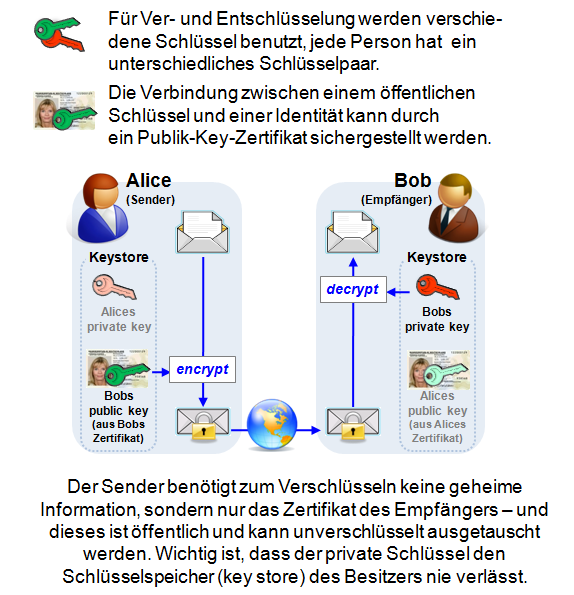
\includegraphics[scale=0.7]{figures/AsymmetricEnc_Figure_Chap1_de.png}
\caption{Asymmetrische oder Public-Key-Verschlüsselung}
\label{cm_Figure_Asymmetric-Enc_Public-Key-Enc}
\end{center}
\end{figure}

Möchte Alice\index{Alice}%
\footnote{%
  Zur Beschreibung kryptographischer Protokolle werden den Teilnehmern
  oft Namen gegeben (vergleiche \cite[S. 23]{Schneier1996}).
  Alice und Bob\index{Bob} führen alle allgemeinen 2-Personen-Protokolle durch,
  wobei Alice dies initiiert und Bob antwortet.
  Die Angreifer werden als Eve (eavesdropper = passiver Lauscher) und
  Mallory (malicious active attacker = böswilliger, aktiver Abgreifer)
  bezeichnet.
  }
mit Bob kommunizieren, so sucht sie Bobs öffentlichen Schlüssel
und benutzt ihn, um ihre Nachricht an ihn zu
verschlüsseln. Diesen verschlüsselten Text schickt sie dann an Bob,
der mit Hilfe seines geheimen Schlüssels den Text wieder entschlüs"-seln
kann. Da einzig Bob Kenntnis von seinem geheimen Schlüssel hat, ist
auch nur er in der Lage, an ihn adressierte Nachrichten zu
entschlüsseln.
Selbst Alice als Absenderin der Nachricht kann aus der von ihr
versandten (verschlüsselten) Nachricht den Klartext nicht wieder
herstellen. Natürlich muss sichergestellt sein, dass man aus dem
öffentlichen Schlüssel nicht auf den geheimen Schlüssel schließen
kann.\par \vskip + 3pt

% Abbildung evtl. besser hier, wenn Seitenaufteilung ausginge.

Veranschaulichen kann man sich ein solches Verfahren mit einer
Reihe von einbruchssicheren Briefkästen. Wenn ich eine Nachricht
verfasst habe, so suche ich den Briefkasten\index{Briefkasten} mit dem
Namensschild des Empfängers und werfe den Brief dort ein. Danach kann ich die
Nachricht selbst nicht mehr lesen oder verändern, da nur der
legitime Empfänger im Besitz des Schlüssels für den Briefkasten
ist.\par \vskip + 3pt

Vorteil von asymmetrischen Verfahren ist das einfachere
\index{Schlüsselmanagement} Schlüsselmanagement. Betrachten wir
wieder ein Netz mit $n$ Teilnehmern. Um sicherzustellen, dass
jeder Teilnehmer jederzeit eine verschlüsselte Verbindung zu
jedem anderen Teilnehmer aufbauen kann, muss jeder Teilnehmer ein
Schlüsselpaar besitzen. Man braucht also $2n$ Schlüssel oder $n$
Schlüsselpaare. Ferner ist im Vorfeld einer Übertragung kein
sicherer Kanal notwendig, da alle Informationen, die zur Aufnahme
einer vertraulichen Kommunikation notwendig sind, offen
übertragen werden können. Hier ist lediglich%
\footnote{%
Dass auch dies nicht trivial ist, wird z.B. in Kapitel \ref{nt_Shared-Primes}
erläutert.
Neben den Anforderungen bei der Schlüsselgenerierung ist zu beachten, dass
inzwischen auch die (Public-Key-)Infrastrukturen selbst Ziel von
Cyber-Angriffen sind.
}
auf die Unverfälschtheit (Integrität und Authentizität)
\index{Authentizität} des öffentlichen Schlüssels zu achten.
Nachteil: Im Vergleich zu symmetrischen Verfahren sind reine
asymmetrische Verfahren jedoch um ein Vielfaches langsamer.\par \vskip + 3pt

Das bekannteste asymmetrische Verfahren ist der \index{RSA}
RSA-Algorithmus\index{CrypTool}%
\footnote{%
  RSA wird in diesem Skript ab Kapitel \ref{rsabeweis} ausführlich beschrieben.
  Die aktuellen Forschungsergebnisse im Umfeld von RSA werden in Kapitel
  \ref{SecurityRSA} beschrieben.
}%
, der nach seinen Entwicklern Ronald \index{Rivest, Ronald} Rivest,
Adi \index{Shamir, Adi} Shamir und Leonard \index{Adleman, Leonard} Adleman
benannt wurde. Der RSA-Algorith"-mus wurde 1978 veröffentlicht.\footnote{%
  Hinweise zur Geschichte von RSA und seiner Veröffentlichung, die nicht im Sinne
  der NSA war, finden sich in der Artikelserie {\em RSA \& Co. in der Schule:
  Moderne Kryptologie, alte Mathematik, raffinierte Protokolle}.
  Siehe \cite{Witten2006}, S. 55 ff (\glqq Penible Lämmergeier\grqq).
  \index{RSA \& Co. in der Schule}
}
Das Konzept der asymmetrischen Verschlüsselung wurde erstmals
von Whitfield Diffie \index{Diffie, Whitfield}  und
Martin \index{Hellman, Martin} Hellman in Jahre 1976 vorgestellt.
Heute spielen auch die Verfahren nach
ElGamal \index{ElGamal, Tahir} eine bedeutende Rolle, vor allem die
\index{Schnorr, Claus-Peter} Schnorr-Varianten im \index{DSA} DSA (Digital
\index{Signatur!digital}\index{DSA-Signatur}\index{Signatur!DSA}
Signature Algorithm).

Angriffe gegen asymmetrische Verfahren werden behandelt in\\
- Kapitel~ \ref{Chapter_ElementaryNT}: \hyperlink{Chapter_ElementaryNT}{Elementare Zahlentheorie},\\
- Kapitel~ \ref{Chapter_ModernCryptography}:
  \hyperlink{Chapter_ModernCryptography}{Moderne Kryptographie},\\
- Kapitel~ \ref{Chapter_EllipticCurves}:
  \hyperlink{Chapter_EllipticCurves}{Elliptische Kurven} und\\
- Kapitel \ref{Chapter_Dlog-FactoringDead}: \hyperlink{Chapter_Dlog-FactoringDead}
  {Aktuelle Resultate zum Lösen diskreter Logarithmen und zur Faktorisierung}.



% --------------------------------------------------------------------------
\newpage
\section[Hybridverfahren]{Hybridverfahren\footnotemark}
\footnotetext{%
   In CT1\index{CT1} finden Sie dieses Verfahren über das Menü
   \textbf{Ver-/Entschlüsseln \textbackslash{} Hybrid}:
   Dabei können Sie die einzelnen Schritte und ihre Abhängigkeiten mit konkreten
   Zahlen nachvollziehen. Die Variante mit RSA als asymmetrischem Verfahren
   ist graphisch visualisiert; die Variante mit ECC nutzt die Standard-Dialoge.
   In beiden Fällen wird AES als symmetrisches Verfahren eingesetzt.\index{AES}\\
   JCT\index{JCT} bietet Hybrid-Verfahren (z.B. ECIES) in der
   Algorithmen-Perspektive an unter \textbf{Algorithms \textbackslash{} Hybrid Ciphers}.
}
\label{CM_Hybrid-procedures}
\index{Hybridverfahren}

Um die Vorteile von symmetrischen und asymmetrischen Techniken gemeinsam
nutzen zu können, werden (zur Verschlüsselung) in der Praxis meist
Hybridverfahren \index{Verschlüsselung!hybrid} verwendet.\par \vskip + 3pt

Hier werden die Mengen-Daten mittels symmetrischer Verfahren
verschlüsselt: Der Schlüssel ist ein vom Absender zufällig\footnote{%
   Die Erzeugung zufälliger Zahlen\index{Zufall} ist ein wichtiger Bestandteil
   kryptographisch sicherer Verfahren.\\
   - Mit CT1\index{CT1} können Sie über das Menü
   \textbf{Einzelverfahren \textbackslash{} Zufallsdaten erzeugen}
   verschiedene Zufallszahlengeneratoren\index{Zufallsgenerator} (PRNGs) ausprobieren.
   Über das Menü \textbf{Analyse \textbackslash{} Zufallsanalyse} können Sie
   verschiedene Testverfahren für Zufallsdaten auf binäre Dokumente
   anwenden.\\
   % CT1 konzentriert sich auf kryptographisch starke
   % \textbf{Pseudo}zufallszahlengeneratoren. \glqq Echte\grqq~
   % Zufallsquellen werden nur über den Aufruf des Secude-Generators einbezogen.\\
   %
   - In CT2\index{CT2} können Sie im Startcenter
   mit dem Suchstring \glqq Zufall\grqq~Vorlagen (Templates) finden, die
   Zufallsgeneratoren\index{Zufallsgenerator} (PRNGs)
   nutzen. Die PRNGs nutzen intern bspw. Keccak\index{Keccak} oder den
   Linear Congruential Generator (LCG)\index{LCG}. Sie werden dann
   bspw. für Schlüsselgenerierung oder Dezimalisierung genutzt.\\
   %
   - JCT\index{JCT} bietet \textbf{Pseudo}zufallszahlengeneratoren sowohl
   im Menü \textbf{Algorithms \textbackslash{} Random Number Generator} der
   Standard-Perspektive als auch in der Algorithmen-Perspektive an.
}\index{Zufall}
generierter geheimer Sitzungsschlüssel (session key)\index{Session Key},
der nur für diese Nachricht verwendet wird.

Anschließend wird dieser Sitzungsschlüssel mit Hilfe des asymmetrischen
Verfahrens verschlüsselt und zusammen mit der Nachricht an den Empfänger
übertragen.

Der Empfänger kann den Sitzungsschlüssel mit Hilfe seines geheimen
Schlüssels bestimmen und mit diesem dann die Nachricht entschlüsseln.

Auf diese Weise profitiert man von dem bequemen Schlüsselmanagement\index{Schlüsselmanagement}
asymmetrischer Verfahren (mit öffentlichem und privatem Schlüssel), und
man profitiert von der Schnelligkeit symmetrischer Verfahren, um große
Datenmengen zu verschlüsseln (mit den geheimen Schlüsseln).



% --------------------------------------------------------------------------
\newpage
% \vskip +40 pt

\begin{ctsquote}
    Ein altes Sprichwort, angeblich geprägt von der
    US National Security Agency (NSA), sagt:\\
    \glqq Angriffe werden immer besser, niemals schlechter.\grqq\\
    ``Attacks always get better; they never get worse.''
\caption[IETF]{IETF\footnotemark}
\end{ctsquote}
\addtocounter{footnote}{0}\footnotetext{%
  \url{http://tools.ietf.org/html/rfc4270}\index{IETF}\index{NSA}
  }

% --------------------------------------------------------------------------
\section[Kryptoanalyse und symmetrische Chiffren für Lehrzwecke]{Kryptoanalyse und symmetrische Chiffren für Lehrzwecke\footnotemark}
\footnotetext{%
  Ein sehr guter Start in die Kryptoanalyse ist das Buch von Mark Stamp \cite{Stamp2007}.
  Ebenfalls gut, aber sehr high-level und nur bezogen auf die Analyse symmetrischer
  Blockchiffren ist der Artikel von Bruce Schneier \cite{Schneier2000}.\\
  Einige der Cipher-Challenges bei \glqq MysteryTwister C3\grqq~
  (\url{http://www.mysterytwisterc3.org}) sind ebenfalls gut für Lehrzwecke
  einsetzbar.\index{MTC3}\index{Krypto-Wettbewerb}
}
\label{CM_Analysis-SymCiphers-Educational}
\index{Kryptoanalyse}

Verglichen mit den auf der Zahlentheorie beruhenden Public-Key-Verschlüsselungsverfahren wie RSA, ist die Struktur von AES\index{AES} und den meisten anderen modernen symmetrischen Verschlüsse"-lungsverfahren (wie DES, IDEA oder Present) sehr komplex und kann nicht so einfach wie RSA\index{RSA} erklärt werden.

Deshalb wurden zu Lehrzwecken vereinfachte Varianten moderner
symmetrischer Verfahren entwickelt, um Einsteigern die Möglichkeit zu geben,
Ver- und Entschlüsselung von Hand zu lernen und ein besseres Verständnis zu
gewinnen, wie die Algorithmen im Detail funktionieren.
Diese vereinfachten Varianten helfen auch, die entsprechenden
Kryptoanalyse-Methoden zu verstehen und anzuwenden.

Die bekanntesten Varianten sind SDES (Simplified DES)%
\footnote{
  Visualisierung: Macht man in CT2\index{CT2} einen Doppelklick auf den Titel der
  SDES-Komponente, ist in der Fullscreen-Ansicht
  % fullscreen
  % in der Fullscreen-Ansicht  %% das gab eine Zeile zuviel und rückte 1.7. weiter.
  zu sehen, wie die Bits der eingegebenen Daten durch den Algorithmus fließen.
  Ein Screen\-shot dazu:
  \url{https://www.facebook.com/CrypTool2/photos/a.505204806238612.1073741827.243959195696509/597354423690316}
}
und S-AES (Simplified-AES) von Prof. Ed Schaefer und seinen Studenten%
\footnote{
    Siehe auch den Artikel \glqq Devising a Better Way to Teach and Learn
    the Advanced Encryption Standard\grqq~unter
    \url{http://math.scu.edu/~eschaefe/getfile.pdf}
    % be_2016-07-17: dead link /toter Link: http://www.scu.edu/cas/research/cryptography.cfm
},
und Mini-AES (siehe das Kapitel~\ref{CM_Sage_Mini-AES} \glqq \nameref{CM_Sage_Mini-AES}\grqq):

\index{DES}\index{DES!SDES}\index{IDEA}\index{AES!Mini-AES}\index{AES!S-AES}
\begin{itemize}

\item Edward F. Schaefer: {\em A Simplified Data Encryption Standard Algorithm}
      \cite{Schaefer1996}.

\item Raphael Chung-Wei Phan: {\em Mini Advanced Encryption Standard (Mini-AES):
                                   A Testbed for Cryptanalysis Students}
      \cite{Phan2002}.

\item Raphael Chung-Wei Phan: {\em Impossible differential cryptanalysis of Mini-AES}
      \cite{Phan2003}.

\item Mohammad A. Musa, Edward F. Schaefer, Stephen Wedig:
      {\em A simplified AES algorithm and its linear and differential cryptanalyses}
      \cite{Musa2003}.

\item Nick Hoffman: {\em A SIMPLIFIED IDEA ALGORITHM}
      \cite{Hoffman2006}.

\item S. Davod. Mansoori, H. Khaleghei Bizaki:
      {\em On the vulnerability of Simplified AES Algorithm Against Linear Cryptanalysis}
      \cite{Mansoori2007}.

\end{itemize}



% --------------------------------------------------------------------------
\section{Weitere Informationsquellen}

Neben den anderen Kapiteln in diesem Skript, der umfangreichen Fachliteratur
und vielen Stellen im Internet enthält auch die Online-Hilfe aller
CrypTool-Varianten\index{CrypTool} sehr viele weitere Informationen zu den
einzelnen symmetrischen und asymmetrischen Verschlüsselungsverfahren.




% ---------------------------------------------------------------------------
% ---------------------------------------------------------------------------
\newpage
\hypertarget{CM_Appendix_SageCode}{}
\section{Anhang: Beispiele mit SageMath}
\label{CM_Sage_samples}
\index{SageMath!Programmbeispiele}

Der folgende Abschnitt enthält SageMath Source-Code, der sich auf den
Inhalt des Kapitels~\ref{CM_Analysis-SymCiphers-Educational}
(\glqq \nameref{CM_Analysis-SymCiphers-Educational}\grqq) bezieht.

Weitere Details zu in SageMath enthaltenen Kryptoverfahren (z.B. zum Simplified
Data Encryption Standard SDES) finden sich z.B. in der Diplomarbeit von Minh Van
Nguyen \cite{Nguyen2009b}.

% ---------------------------------------------------------------------------
\subsection{Mini-AES}
\label{CM_Sage_Mini-AES}
\index{AES!Mini-AES}

Das SageMath-Modul \texttt{crypto/block\_cipher/miniaes.py} enthält den Mini-AES, mit
dem Studenten die Funktionsweise moderner Blockchiffren untersuchen können.

Mini-AES, ursprünglich vorgestellt von \cite{Phan2002}, ist eine vereinfachte
Variante des Advanced Encryption Standard (AES) für Ausbildungszwecke.

Wie man Mini-AES benutzt, ist ausführlich in der SageMath Reference-Page beschrieben:
\begin{sloppypar} % Nötig, da sonst ein schwarzer Punkt
  \url{http://doc.sagemath.org/html/en/reference/cryptography/sage/crypto/block_cipher/miniaes.html}.
\end{sloppypar}

Das folgende SageMath-Code-Beispiel~\ref{cm_Mini-AES:Sage_example}
ist aus den Release-Notes von SageMath 4.1%
\footnote{
  Siehe \url{http://mvngu.wordpress.com/2009/07/12/sage-4-1-released/}.\\
  Weiterer Beispiel-Code zum Mini-AES findet sich in
  \cite[Kap. 6.5 und Anhang D]{Nguyen2009a}.
}
und ruft diese Implementierung des Mini-AES auf.


% Using [fontsize=\footnotesize,fontshape=tt] caused:
%   LaTeX Font Warning: Font shape `T1/cmtt/m/tt' undefined
%   (Font)              using `T1/cmtt/m/n' instead on input line 730.
% so deleted the fontshape parameter.
\begin{sagecode}
\begin{Verbatim}%
[fontsize=\footnotesize]
# We can encrypt a plaintext using Mini-AES as follows:
sage: from sage.crypto.block_cipher.miniaes import MiniAES
sage: maes = MiniAES()
sage: K = FiniteField(16, "x")
sage: MS = MatrixSpace(K, 2, 2)
sage: P = MS([K("x^3 + x"), K("x^2 + 1"), K("x^2 + x"), K("x^3 + x^2")]); P

[  x^3 + x   x^2 + 1]
[  x^2 + x x^3 + x^2]
sage: key = MS([K("x^3 + x^2"), K("x^3 + x"), K("x^3 + x^2 + x"), K("x^2 + x + 1")]); key

[    x^3 + x^2       x^3 + x]
[x^3 + x^2 + x   x^2 + x + 1]
sage: C = maes.encrypt(P, key); C

[            x       x^2 + x]
[x^3 + x^2 + x       x^3 + x]

# Here is the decryption process:
sage: plaintxt = maes.decrypt(C, key)
sage: plaintxt == P
True

# We can also work directly with binary strings:
sage: from sage.crypto.block_cipher.miniaes import MiniAES
sage: maes = MiniAES()
sage: bin = BinaryStrings()
sage: key = bin.encoding("KE"); key
0100101101000101
sage: P = bin.encoding("Encrypt this secret message!")
sage: C = maes(P, key, algorithm="encrypt")
sage: plaintxt = maes(C, key, algorithm="decrypt")
sage: plaintxt == P
True

# Or work with integers n such that 0 <= n <= 15:
sage: from sage.crypto.block_cipher.miniaes import MiniAES
sage: maes = MiniAES()
sage: P = [n for n in xrange(16)]; P
[0, 1, 2, 3, 4, 5, 6, 7, 8, 9, 10, 11, 12, 13, 14, 15]
sage: key = [2, 3, 11, 0]; key
[2, 3, 11, 0]
sage: P = maes.integer_to_binary(P)
sage: key = maes.integer_to_binary(key)
sage: C = maes(P, key, algorithm="encrypt")
sage: plaintxt = maes(C, key, algorithm="decrypt")
sage: plaintxt == P
True
\end{Verbatim}
\caption{Ver- und Entschlüsselung mit dem Mini-AES}
\label{cm_Mini-AES:Sage_example}
\end{sagecode}
\clearpage%% Um das Codebeispiel vor das ff. Kap. 1.8.2 zu bekommen.


% ---------------------------------------------------------------------------
\subsection{Weitere symmetrische Krypto-Algorithmen in SageMath}
\label{CM_Sage_SymCryptoAlg}

Die Referenz zu SageMath v8.2 führt als kryptographische Funktionen u.a. auf:%
\footnote{
  Siehe
  \url{http://doc.sagemath.org/html/en/reference/sage/crypto/index.html},\\
  \url{http://doc.sagemath.org/html/en/reference/cryptography/index.html} und\\
  \url{http://doc.sagemath.org/html/en/reference/cryptography/sage/crypto/stream.html}
}
\begin{itemize}
   \item Linear feedback shift register (LFSR),
   \item Blum-Blum-Shub (BBS): Pseudo-Zufallsbit-Generator (zu finden bei Streams),
   \item Gitter-basierte Funktionen.
% be_2016-07-17: Nicht mehr gefunden in Refrence 7.2:
% - ShrinkingGeneratorCryptosystem,
\end{itemize}



%------------------------------------------------------------------------------

\printbibliography[%
	heading=subbibintoc,
	title={Literatur zu Kapitel \thechapter},
	segment=\therefsegment,
]

Alle Links wurden am 10.07.2016 überprüft.



% --------------------------------------------------------------------------
\newpage
\chapter*{Web-Links}\addcontentsline{toc}{section}{Web-Links}

\begin{enumerate}

  \hypertarget{CM_HT_Weblink_Rijndael-Cryptosystem}{}
  \item \glqq AES Discussion Groups\grqq~beim NIST (archive page provided for historical purposes, last update on Feb 28th, 2001)\\
	% \grqq nach \item braucht die Tilde, aber kein weiteres Blank.
	%  Sonst reicht ein Blank, wenn ein weiteres Wort danach folgt
	%  (es reicht auch nicht, wenn danach ein Zeilenumbruch).
	\url{https://csrc.nist.gov/archive/aes/}

  \item Das AES-/Rijndael-Kryptosystem (page maintained by Nicolas T. Courtois, last update on Aug 24th, 2007)\\
        \url{http://www.cryptosystem.net/aes}

  \item distributed.net:~\glqq RC5-64 has been solved\grqq\\
        \url{http://www.distributed.net/Pressroom_press-rc5-64}

	% \begin{sloppypar}  ... \end{sloppypar} worked. Get rid of \\ before to avoid extra newline.
\item RSA Labs (ehemals RSA Security): ~\glqq The RSA Secret Key Challenge\grqq
        \begin{sloppypar}
	\url{https://www.emc.com/emc-plus/rsa-labs/historical/the-rsa-laboratories-secret-key-challenge.htm}
	\end{sloppypar}

  \item RSA Labs (ehemals RSA Security): ~\glqq DES Challenge\grqq\\
        \url{https://www.emc.com/emc-plus/rsa-labs/historical/des-challenge-iii.htm}

  \item Weiterführende Links auf der CrypTool-Homepage\\
        \url{http://www.cryptool.org}
	
\end{enumerate}

Alle Links wurden am 06.08.2018 überprüft.

\end{refsegment}

% Local Variables:
% TeX-master: "../script-de.tex"
% End:
